\documentclass[11pt]{exam}
% \usepackage{pslatex}
\usepackage{xparse}
\usepackage{graphicx}
\DeclareGraphicsExtensions{.jpg, .png}
\usepackage{amsmath}
%\usepackage{amsfonts}
\usepackage{fourier,MnSymbol}
\usepackage{enumerate}
\firstpageheader{}{}{}
\runningheader{\textbf{Spring 2013}}
 {}
 {\textbf{Math 352}}
 %{\emph{Page \thepage~of \numpages}}
\runningheadrule
\setlength{\parskip}{1ex}
\setlength{\parindent}{0pt}
\pagestyle{head}
%\newcommand{\N}{\mathbb{N}}
%\newcommand{\Z}{\mathbb{Z}}
%\newcommand{\R}{\mathbb{R}}
%\newcommand{\dwrspace}[1]{\vspace*{\stretch{#1}}}
\NewDocumentCommand\N{}{\mathbf{N}}
\NewDocumentCommand\R{}{\mathbf{R}}
\NewDocumentCommand\Z{}{\mathbf{Z}}
\NewDocumentCommand\Q{}{\mathbf{Q}}
\NewDocumentCommand\dwrspace{m}{\vspace*{\stretch{#1}}}
\begin{document}
\noindent
\textbf{{\large Mathematics 352 \\ Quiz 1}}
% \hfill Name: \underline{\hspace{0.5in}Answers\hspace{2in}}

\noindent
February 13, 2013; 5 minutes  \hfill Name: \underline{\hspace{3in}} 

\begin{questions}  

\question Match the differential equations to the corresponding slope fields by writing the letter of your choice on the slope field it matches.
    \begin{choices}
        \item $y' = 3y - y^2$
        \item $y' = y - 2$
        \item $y' = 2 - y$
        \item $y' = y^2 - 3y$
    \end{choices}
\begin{figure}[ht]
    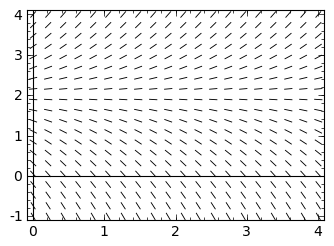
\includegraphics[width = 0.45\linewidth]{sage0} \hspace{0.08\linewidth}
    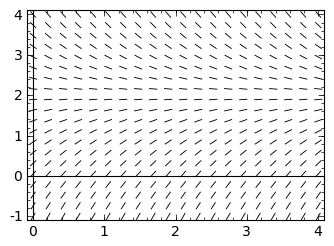
\includegraphics[width = 0.45\linewidth]{sage1}
        
    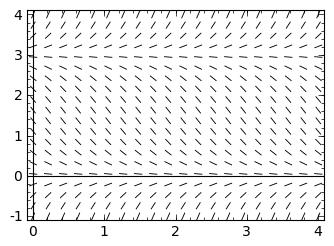
\includegraphics[width = 0.45\linewidth]{sage2} \hspace{0.08\linewidth}
    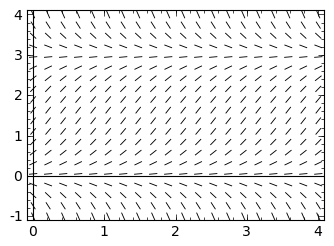
\includegraphics[width = 0.45\linewidth]{sage3}
\end{figure}
% \begin{figure}[ht]
%     \begin{minipage}[t]{0.3\linewidth}
%         \begin{choices}
%             \item $y' = 3y - y^2$
%             \item $y' = y - 2$
%             \item $y' = 2 - y$
%             \item $y' = y^2 - 3y$
%         \end{choices}
%     \end{minipage}
%     \hspace{0.05\linewidth}
%     \begin{minipage}{0.6\linewidth}
%         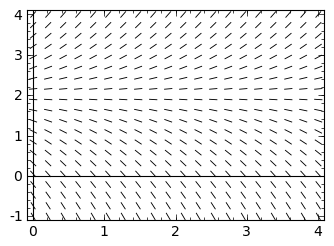
\includegraphics[width = 0.45\linewidth]{sage0} \hspace{0.08\linewidth}
%         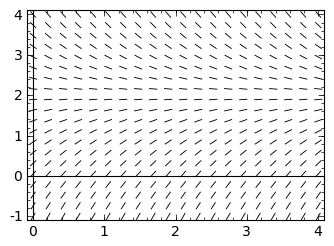
\includegraphics[width = 0.45\linewidth]{sage1}
        
%         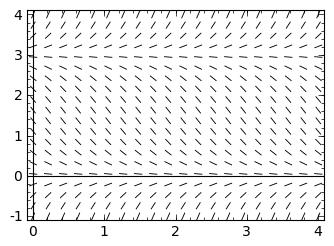
\includegraphics[width = 0.45\linewidth]{sage2} \hspace{0.08\linewidth}
%         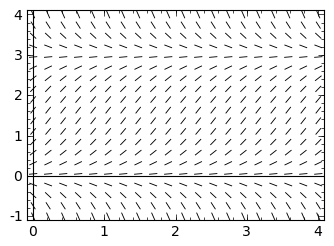
\includegraphics[width = 0.45\linewidth]{sage3}
%     \end{minipage}
% \end{figure}

\dwrspace{1}


\end{questions}

\end{document}